%----------------------------------------------------------------------------------------
%	PACKAGES AND THEMES
%----------------------------------------------------------------------------------------
\documentclass[aspectratio=169,xcolor=dvipsnames,7pt]{beamer}
\usetheme{Simple}

\usepackage[spanish]{babel}
\usepackage{hyperref}
\usepackage{graphicx} % Allows including images
\usepackage{booktabs} % Allows the use of \toprule, \midrule and \bottomrule in tables
\usepackage{tikz}
\usepackage{physics}

% import citation 
\usepackage[style=numeric,backend=biber,autocite=footnote]{biblatex}
\addbibresource{references.bib}
\setbeamerfont{footnote}{size=\tiny}

%----------------------------------------------------------------------------------------
%	TITLE PAGE
%----------------------------------------------------------------------------------------

% The title
\title[]{Rotor pateado}
% \subtitle{Subtitle}

\author[]{José Alfredo de León}
\institute[] % Your institution may be shorthand to save space
{
    % Your institution for the title page
%    \vskip 3pt
}
\date{\large \today} % Date, can be changed to a custom date


%----------------------------------------------------------------------------------------
%	PRESENTATION SLIDES
%----------------------------------------------------------------------------------------


\begin{document}

\begin{frame}
    % Print the title page as the first slide
    \titlepage
    Si alguna vez se vuelven a usar estas diapositivas tomar en cuenta para hacer cambios que
    \begin{itemize}
    \item $k_C$ no es el parámetro que regula caoticidad, el sistema siempre es caótico
    \item Antes de $k_C$ todavía existen curvas en el espacio de fase que acotan espacios caóticos (espacios punteados), después del valor crítico ya cualquier cosa puede pasar
    \end{itemize}
\end{frame}

%\begin{frame}{Overview}
%    % Throughout your presentation, if you choose to use \section{} and \subsection{} commands, these will automatically be printed on this slide as an overview of your presentation
%    \tableofcontents
%\end{frame}

\begin{frame}{¿Qué es un diagrama de fase?}

\begin{columns}
\begin{column}{0.55\textwidth}  %%<--- here
El espacio de fase es el espacio en el que viven todos los posibles estados
de un sistema.\footnote[frame]{\fullcite{nathanson2007pauli}}

\vspace*{.5cm}
Por ejemplo, el espacio de fase del oscilador armónico simple (OAS) 
es el espacio de las variables canónicas $q$ y $p$, que como es 2D lo podemos
graficar.

\vspace*{.5cm} 
La manera pedestre de dibujar el espacio de fase es obtener con nuestro
formalismo favorito las ecuaciones de movimiento, resolverlas y dibujar
punto a punto $\big(q(t),p(t)\big)$ para diferentes condiciones iniciales.
\end{column}

\hspace*{-1.5cm}
\begin{column}{0.4\textwidth}  %%<--- here
\begin{figure}
\includegraphics[width=\textwidth]{oas_pedestre}
\end{figure}
\end{column}
\end{columns}
\end{frame}


\begin{frame}[allowframebreaks]{Diagramas de fase $q$-$p$: oscilador armónico}


\begin{columns}
\begin{column}{0.59\textwidth}  %%<--- here
El OAS está descrito por el Hamiltoniano
\begin{align*}
\only<1>{H = \frac{p^2}{2} + \frac{q^2}{2}}\quad (m=k=1),
\only<3>{\alert{\frac{p^2}{2} + \frac{q^2}{2}= E}}
\end{align*}
del cual se calculan sus ecuaciones de movimiento:
\begin{align*}
\dot q &= \pdv{H}{p}, & \dot p &= - \pdv{H}{q} \\
\dot q &=p & \dot p &=-q,
\end{align*}
con esto podemos dibujar el diagrama de direcciones/fase, 
usando $\dot p/\dot q = dp/dq = -q/p$. \vspace*{.5cm}

O también podemos dibujar las \alert{trayectorias de energía constante}
$p^2/2+q^2/2=E$.
\end{column}

\hspace*{-1.5cm}
\begin{column}{0.4\textwidth}  %%<--- here
\begin{figure}
\includegraphics[width=\textwidth]{oas}
\end{figure}

\end{column}
\end{columns}

\framebreak

\begin{columns}[t]
\begin{column}{0.5\textwidth}  %%<--- here
\vspace*{1cm}

Consideremos un oscilador más general:
\begin{align*}
&& \ddot q + 2\xi\dot q + q &= 0,\quad (m=1)
\end{align*}
de donde podemos calcular el diagrama de direcciones con
\begin{align*}
\frac{\dot p}{\dot q} = \frac{dp}{dq} = -2\xi - q/p.
\end{align*} 
\end{column}

\hspace*{-1cm}
\begin{column}{0.5\textwidth}  %%<--- here
\vspace*{-.9cm}
\begin{figure}
\includegraphics[height=.45\textheight]{oas_05}
\includegraphics[height=.45\textheight]{oas_02}

\includegraphics[height=.45\textheight]{oas_03}
\includegraphics[height=.45\textheight]{oas_04}
\end{figure}

\end{column}
\end{columns}
\end{frame}

\begin{frame}
En conclusión,
\begin{itemize}
\item Para estudiar la dinámica de un sistema podemos estudiar las trayectorias en el espacio de fases
\item Los diagramas de fases nos permiten ver varias cosas interesantes sobre
la dinámica de un sistema, que al \textit{ojímetro} no vemos de las solución a las ecuaciones de movimiento
\item El OAS es un \alert{sistema integrable}, i.e. tiene trayectorias bien definidas en el espacio de fase
\end{itemize}

\vspace*{1cm}
¿Cómo podemos identificar caos en el espacio de fases? Trayectorias no definidas.
\end{frame}

%------------------------------------------------
\section{First Section}
%------------------------------------------------

\begin{frame}{Ahora sí, el rotor pateado}
\begin{columns}
\begin{column}{0.5\textwidth}  %%<--- here
		\vspace*{-.4cm}
    \begin{figure}
     \includegraphics[width=.95\textwidth]{kicked_rotor}
     \vspace*{-5mm}
     \caption{\normalsize Rotor pateado}
     \end{figure}
\end{column}

\begin{column}{0.5\textwidth}
El rotor pateado es un modelo físico, con cierta sencillez, que exhibe caos.\vskip 15pt

El Hamiltoniano del sistema es
\begin{align*}
H = \frac{p^2_{\theta}}{2I} + k\cos\theta\sum_n\delta(t- n \tau),
\end{align*}
con $\delta(\ldots)$ la función delta de Dirac.
\end{column}
\end{columns}
\end{frame}

\begin{frame}{Descripción del sistema}

\begin{columns}
\begin{column}{0.5\textwidth}  %%<--- here
		\vspace*{-.4cm}
    \begin{figure}
     \includegraphics[width=.95\textwidth]{kicked_rotor}
     \vspace*{-5mm}
     \caption{\normalsize Rotor pateado}
     \end{figure}
\end{column}

\begin{column}{0.5\textwidth}
El Hamiltoniano del sistema es
\begin{align*}
H = \frac{p^2_{\theta}}{2I} + k\cos\theta\sum_n\delta(t- n \tau),
\end{align*}
con $\delta(\ldots)$ la función delta de Dirac. \vskip 10pt

Las ecuaciones de movimiento son 
\begin{align*}
\frac{dp_{\theta}}{dt} &= k\sin\theta\sum_n\delta(t - n\tau), \\
\frac{d\theta}{dt} &= \frac{p_{\theta}}{I}.
\end{align*}

\end{column}
\end{columns}

\end{frame}

\begin{frame}{Más descripción del sistema}

\begin{columns}
\begin{column}{0.5\textwidth}  %%<--- here
		\vspace*{-.4cm}
    \begin{figure}
     \includegraphics[width=.95\textwidth]{kicked_rotor}
     \vspace*{-5mm}
     \caption{\normalsize Rotor pateado}
     \end{figure}
\end{column}

\begin{column}{0.5\textwidth}
De las ecuaciones de movimiento  
\begin{align*}
\frac{dp_{\theta}}{dt} &= k\sin\theta\sum_n\delta(t - n\tau) &
\frac{d\theta}{dt} = \frac{p_{\theta}}{I}
\end{align*}
vemos que 
\begin{itemize}
\item entre patadas, i.e. $n\tau<t<(n+1)\tau$, el momentum $p_\theta$ se
conserva
\item cada vez que el sistema recibe una patada el momentum aumenta $k\sin\theta$
\end{itemize}

El sistema está descrito entonces por el mapeo 
\begin{align*}
p_\theta(n+1) &= p_\theta(n) + k\sin\theta(n)\mod{(2\pi)} \\
\theta(n+1) &= \theta(n) + p_\theta(n+1)\mod{(2\pi)}
\end{align*}
\end{column}
\end{columns}

\end{frame}



\begin{frame}{Diagramas de fase del rotor pateado}

\centering

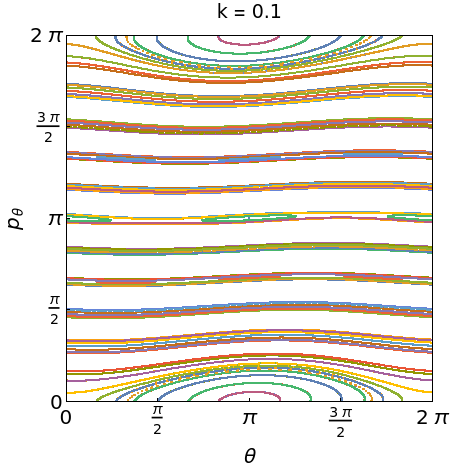
\includegraphics[width=.24\textwidth]{k_0_1.png}
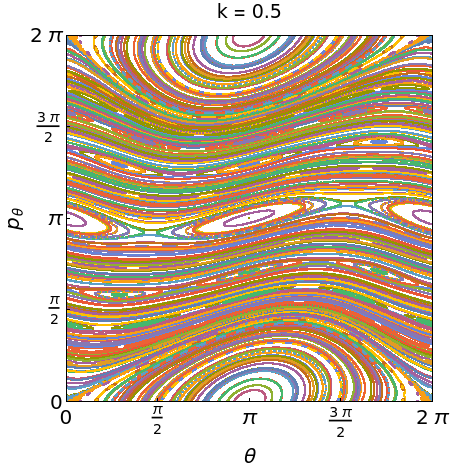
\includegraphics[width=.24\textwidth]{k_0_5.png}
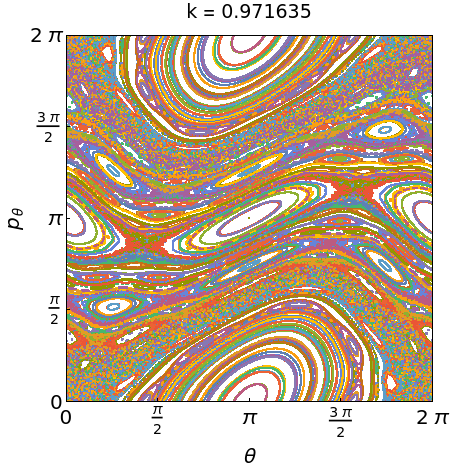
\includegraphics[width=.24\textwidth]{k_0_971635.png}
 	
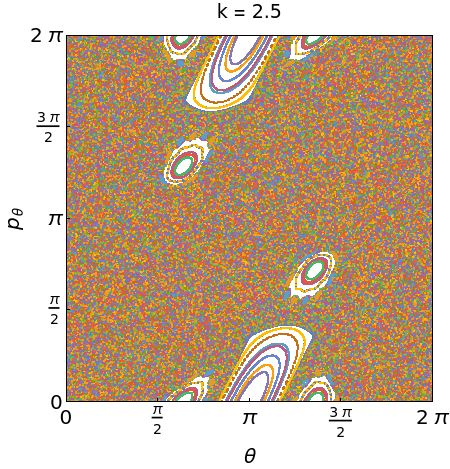
\includegraphics[width=.24\textwidth]{k_2_5.png}
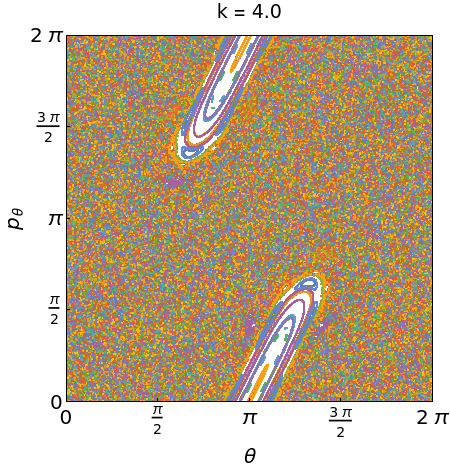
\includegraphics[width=.24\textwidth]{k_4_0.png}
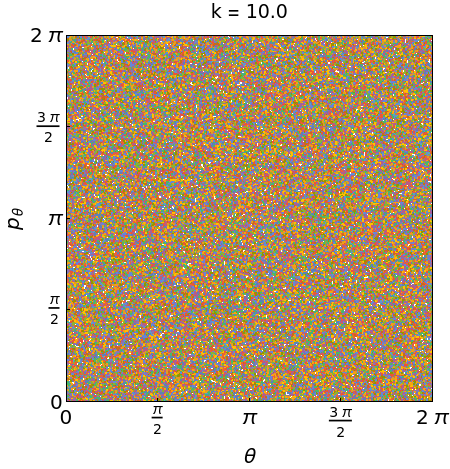
\includegraphics[width=.24\textwidth]{k_10_0.png}


\begin{tikzpicture}[remember picture, overlay]
\node at (7.2,4.8) {\rotatebox{90}{\scriptsize 
El código para hacer estos diagramas está disponible 
%disponible en
}};
\node at (7.55,4.35) {\rotatebox{90}{\scriptsize
%El código para hacer estos diagramas se encuentra 
en \href{https://github.com/deleonja/caos\_cuantico}{https://github.com/deleonja/caos\_cuantico}}};
\end{tikzpicture}
\end{frame}

\begin{frame}[t]{Dos regímenes}
	\begin{columns}
		\begin{column}{0.39\textwidth}  %%<--- here
			\centering
			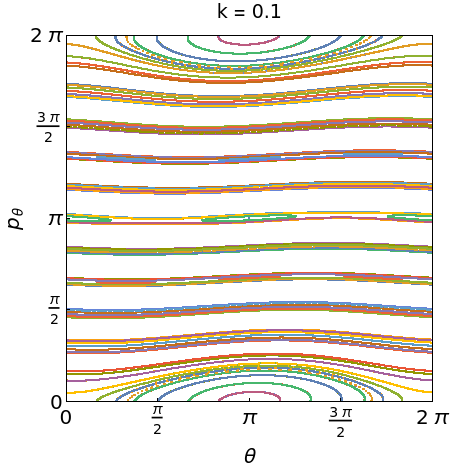
\includegraphics[width=.4\textwidth]{k_0_1.png}
			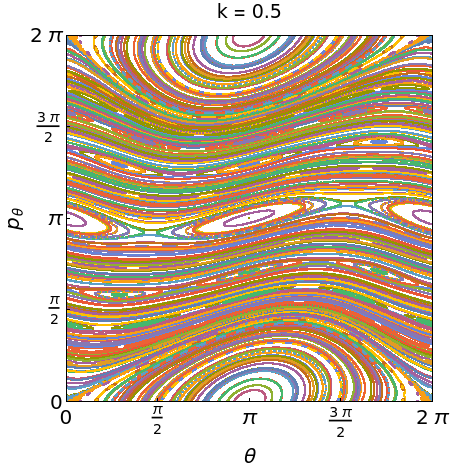
\includegraphics[width=.4\textwidth]{k_0_5.png}
			
			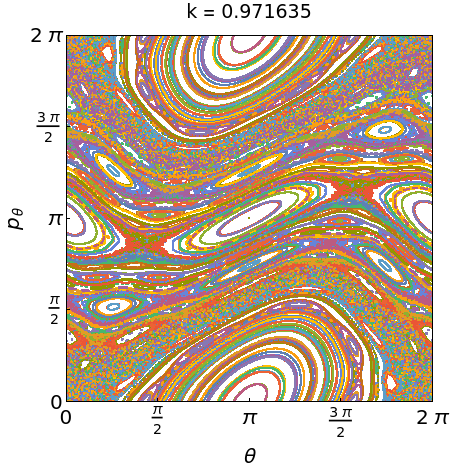
\includegraphics[width=.4\textwidth]{k_0_971635.png}			 	
			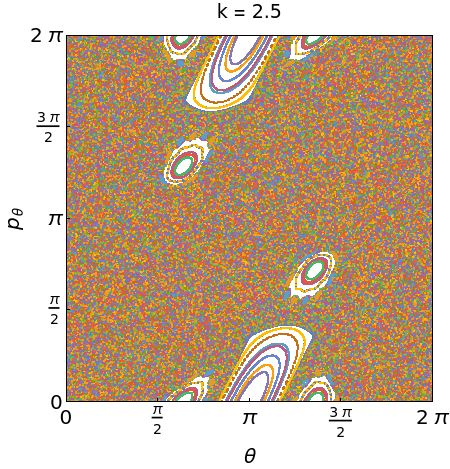
\includegraphics[width=.4\textwidth]{k_2_5.png}
			
			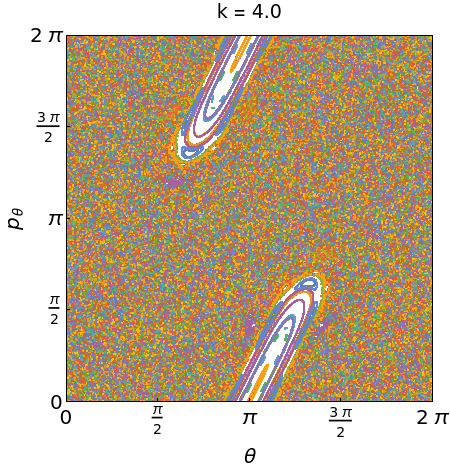
\includegraphics[width=.4\textwidth]{k_4_0.png}
			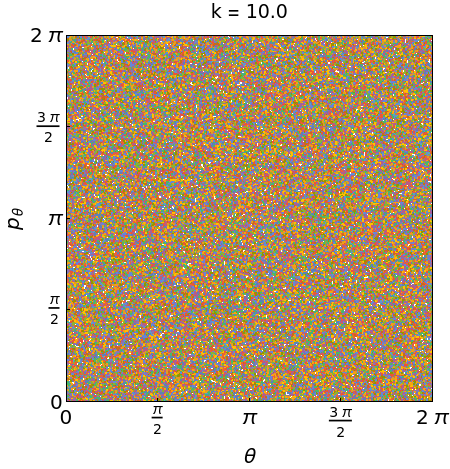
\includegraphics[width=.4\textwidth]{k_10_0.png}
		\end{column}	
		\begin{column}{0.59\textwidth}
			\begin{align*}
				p_\theta(n+1) &= p_\theta(n) + k\sin\theta(n)\mod{(2\pi)} \\
				\theta(n+1) &= \theta(n) + p_\theta(n+1)\mod{(2\pi)}
			\end{align*}
			
			Dos casos:
			\begin{itemize} 
				\item $k<k_c=0.971635\ldots$
				
				Las curvas
				invariantes KAM restringen la variación del momentum a estar acotado
				\item $k>k_c$ 
				
				La variación del momentum $p_\theta$ no está acotada y está 
				caracterizada por un comportamiento difusivo 
			\end{itemize}
		\end{column}
	\end{columns}
\end{frame}

\begin{frame}{Difusión del momentum en el régimen cáotico}
	\begin{columns}
		\begin{column}{0.59\textwidth}  %%<--- here
			\begin{align*}
					p_\theta(n+1) &= p_\theta(n) + k\sin\theta(n)\mod{(2\pi)} \\
					\theta(n+1) &= \theta(n) + p_\theta(n+1)\mod{(2\pi)}
				\end{align*}
			Cuando $k\gg k_c$ cada patada entre $\theta(n)$ y $\theta(n+1)$ 
			es tan fuerte que se pueden
			considerar estadísticamente no correlacionadas. De hecho, se puede comprobar numéricamente que $\expval{p^2}\propto t$.
		\end{column}	
		\begin{column}{0.39\textwidth}
			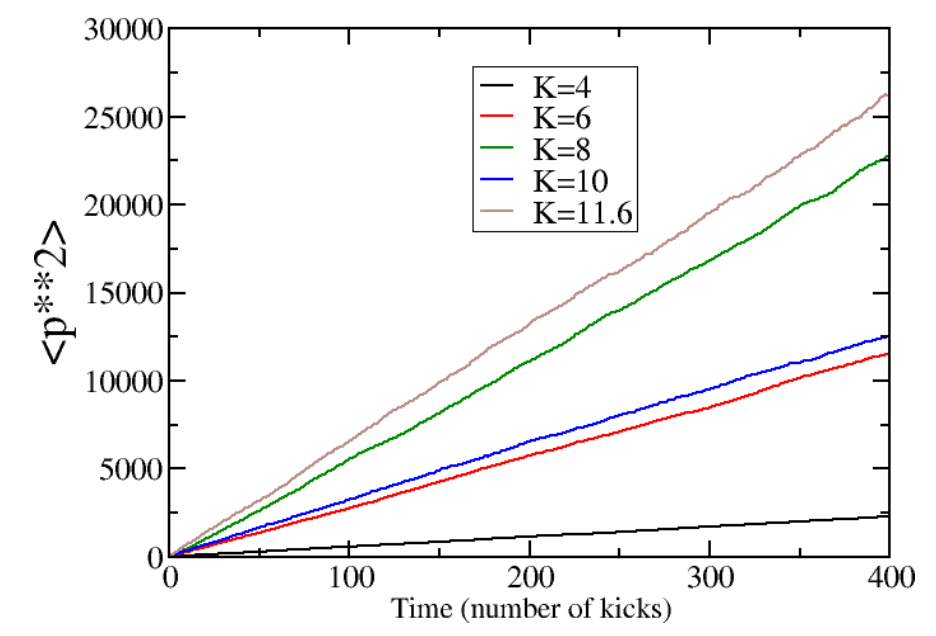
\includegraphics[width=.9\textwidth]{D}
		\end{column}
	\end{columns}
\end{frame}

\begin{frame}
	\begin{columns}
		\begin{column}{0.55\textwidth}  %%<--- here
			Se puede encontonces calcular que $\expval{p^2}=2D_0t$, con 
			\begin{itemize}
				\item $k_c<k<4$: $D_0 \approx (k - k_c)^3/3$
				\item $k>4$: 
				\begin{align*}
					D_0=\frac{k^2}{4}\Big(1 - 2J_2(k) + J_2^2(k)\Big),
				\end{align*}
				con $J_2(k)$ la función de Bessel de primera especie y orden 2.
			\end{itemize}
		\end{column}\hspace*{-5mm}
		\begin{column}{0.49\textwidth}
			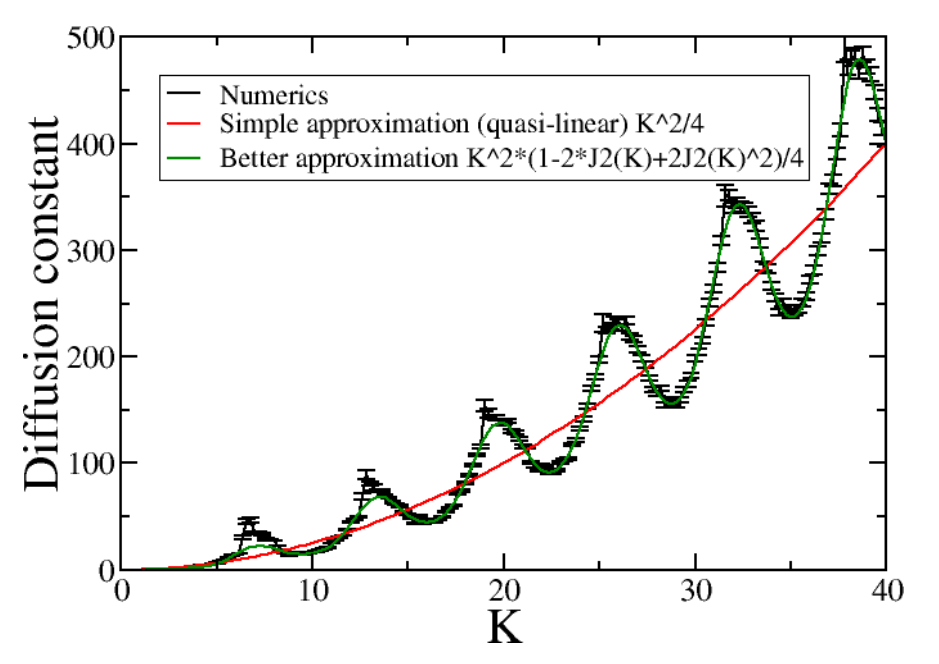
\includegraphics[width=\textwidth]{D3}
		\end{column}
	\end{columns}
\end{frame}

%\begin{frame}{Puntos importantes del valor de $k$}
%\begin{itemize}
%\item Por debajo del parámetro crítico $k_c=0.971635\ldots$ las curvas
%invariantes KAM restringen la variación del momentum a estar acotado. Por encima de este valor, el momentum está caracterizado por un crecimiento difusivo $p^2\approx D_0 t$, con $D_0\approx (k-k_c)^3/3$ para $k_c<4<k$ y $D_0\approx K^2/2$ para $k>4$. 
%\item La curva de oro KAM con número de rotación $r_g=0.618033\ldots$ 
%se destruye en $k=k_c$
%\end{itemize}
%\end{frame}

\begin{frame}{Mapeo estándar de Chirikov}
Más general aún, el mapeo 
\begin{align*}
p_\theta(n+1) &= p_\theta(n) + k\sin\theta\mod{(2\pi)} \\
\theta(n+1) &= \theta(n) + p_\theta(n+1)\mod{(2\pi)}
\end{align*}
se conoce como el mapeo estándar de Chirikov y describe el comportamiento 
universal y genérico de mapeos que preservan el área con espacios de 
fase divididos cuando las islas integrables están rodeadas de componentes
caóticas. \vskip 10pt 

Algunos sistemas que describe son:
\begin{itemize}
%\item Capa caótica alrededor de la separatriz de un resonancia no lineal 
%inducida por una fuerza monocromática
\item Confinamiento de una partícula cargada en trampas de espejo magnéticas 
\item Dinámica de una partícula en un acelerador
\end{itemize}
\end{frame}

\begin{frame}
	\begin{columns}
		\begin{column}{0.39\textwidth}  %%<--- here
				\begin{itemize}
					\item<1-> El rotor pateado es un sistema físico descrito por 
					\begin{align*}
						H = \frac{p^2_{\theta}}{2I} + k\cos\theta\sum_n\delta(t- n \tau)
					\end{align*}
					\item<2-> Según el valor de $k$ por debajo o encima de un valor crítico $k_c$, 
					el sistema exhibe un régimen integrable o caótico
					\item<3-> En el régimen caótico la variación del momentum tiene un comportamiento difusivo
				\end{itemize}
		
		\vspace*{10mm}		
		\only<4->{\centering \Large ¡Gracias!}
		\end{column}	
		\begin{column}{0.59\textwidth}
			\centering
			\only<1>{
			\includegraphics[width=.7\textwidth]{kicked_rotor}
			}
			
			\only<2>{
			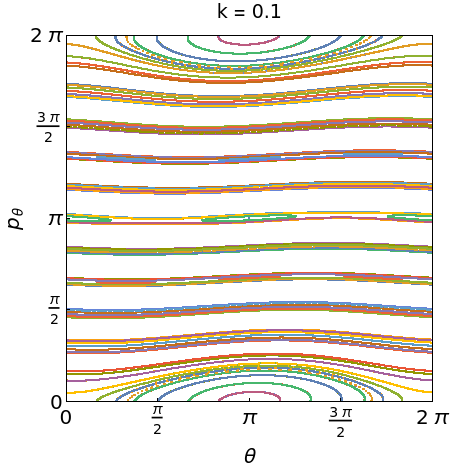
\includegraphics[width=.32\textwidth]{k_0_1.png}
			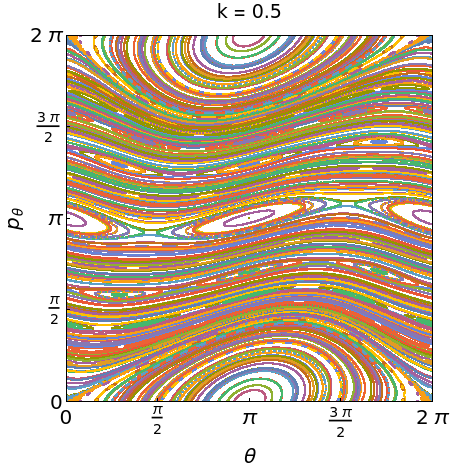
\includegraphics[width=.32\textwidth]{k_0_5.png}
			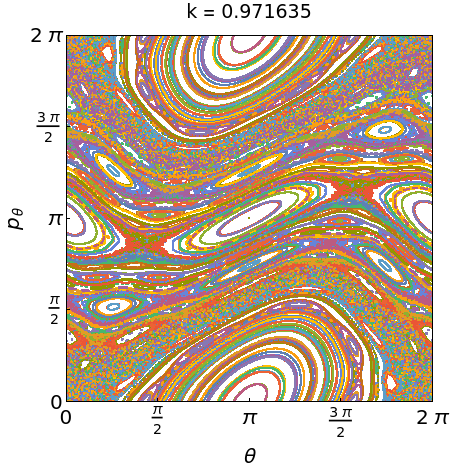
\includegraphics[width=.32\textwidth]{k_0_971635.png}
			 	
			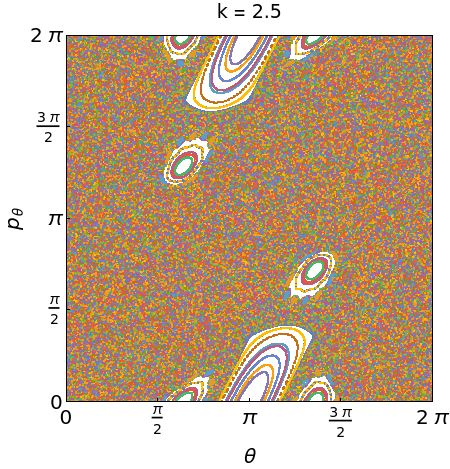
\includegraphics[width=.32\textwidth]{k_2_5.png}
			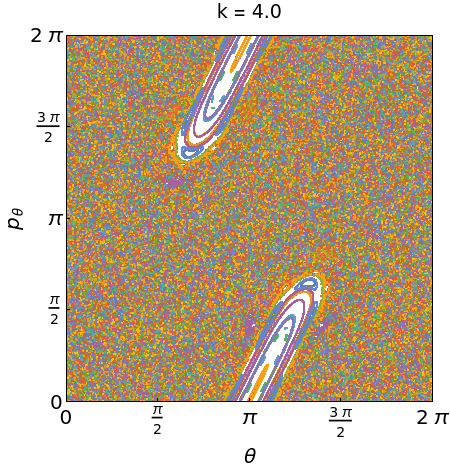
\includegraphics[width=.32\textwidth]{k_4_0.png}
			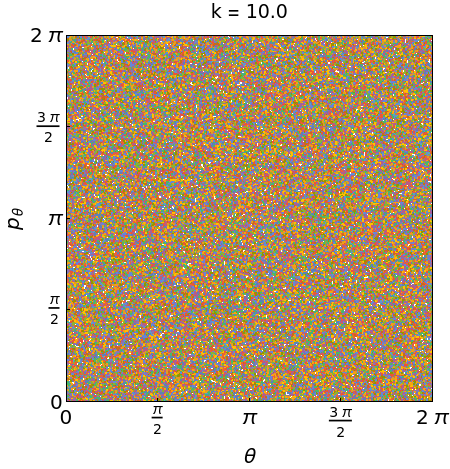
\includegraphics[width=.32\textwidth]{k_10_0.png}
			}
			
			\only<3->{
			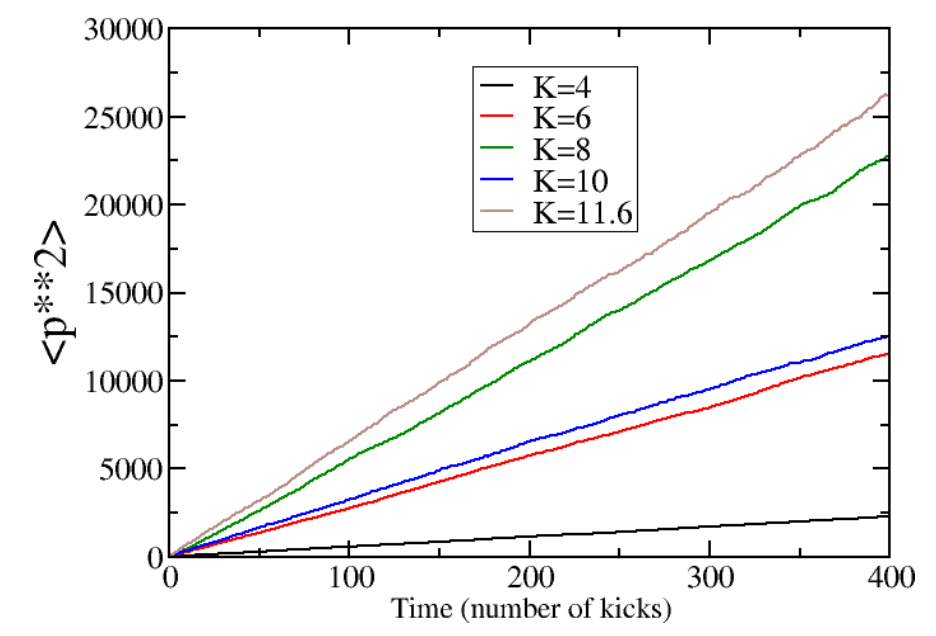
\includegraphics[height=.45\textheight]{D}
			
			\hspace*{3mm}
			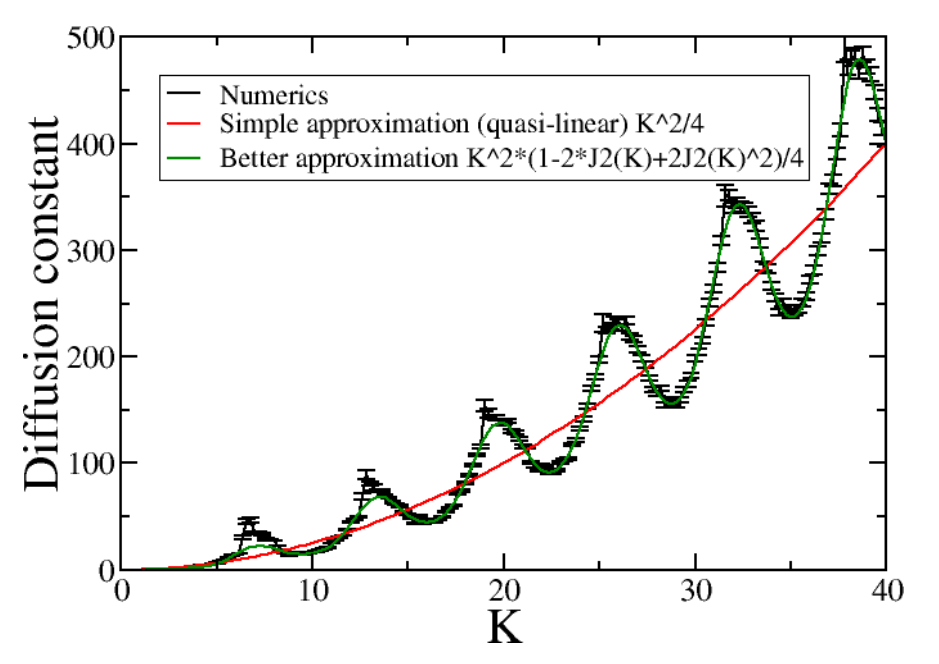
\includegraphics[height=.45\textheight]{D3}
			}
		\end{column}
	\end{columns}
\end{frame}

%------------------------------------------------

%\begin{frame}{References}
%    % Beamer does not support BibTeX so references must be inserted manually as below
%    \footnotesize{
%        \begin{thebibliography}{99}
%            \bibitem[Smith, 2012]{p1} John Smith (2012)
%            \newblock Title of the publication
%            \newblock \emph{Journal Name} 12(3), 45 -- 678.
%        \end{thebibliography}
%    }
%\end{frame}

%------------------------------------------------

%----------------------------------------------------------------------------------------

 \begin{frame}
     \printbibliography
 \end{frame} 

\end{document}